
\section{Hosting Requirements}
This section is applicable if you want to host DemoBot on your own server.

\subsection{Prerequisites}

\subsubsection{Creating The Bot Instance}
\begin{enumerate}

	\item{
		Head over to https://discord.com/developers/applications
	}
	\item{
		Click on the button labelled `New Application` which is located at the top right.\\\\
		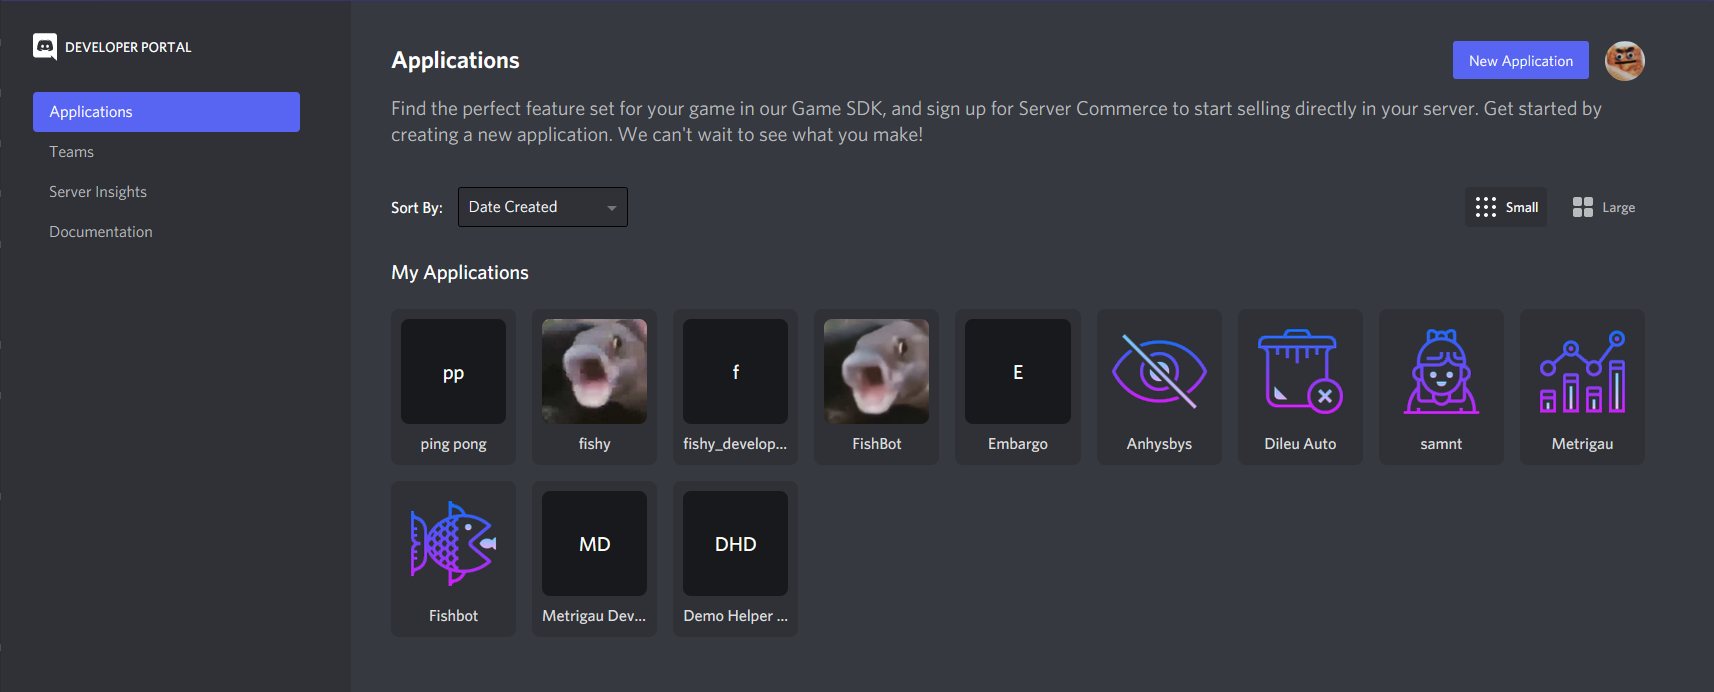
\includegraphics[width=15cm]{hosting_requirements/img1}
	}
	\item{
		Give it a name.
		For example, $Demo Helper$.
	}
	\item{
		Head over to the menu titled $OAuth2$ as seen below:\\\\
		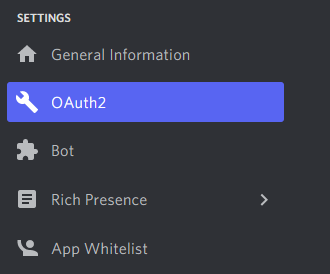
\includegraphics[width=8cm]{hosting_requirements/img2}
	}
	\item{
		Select the checkboxes as seen below:\\\\
		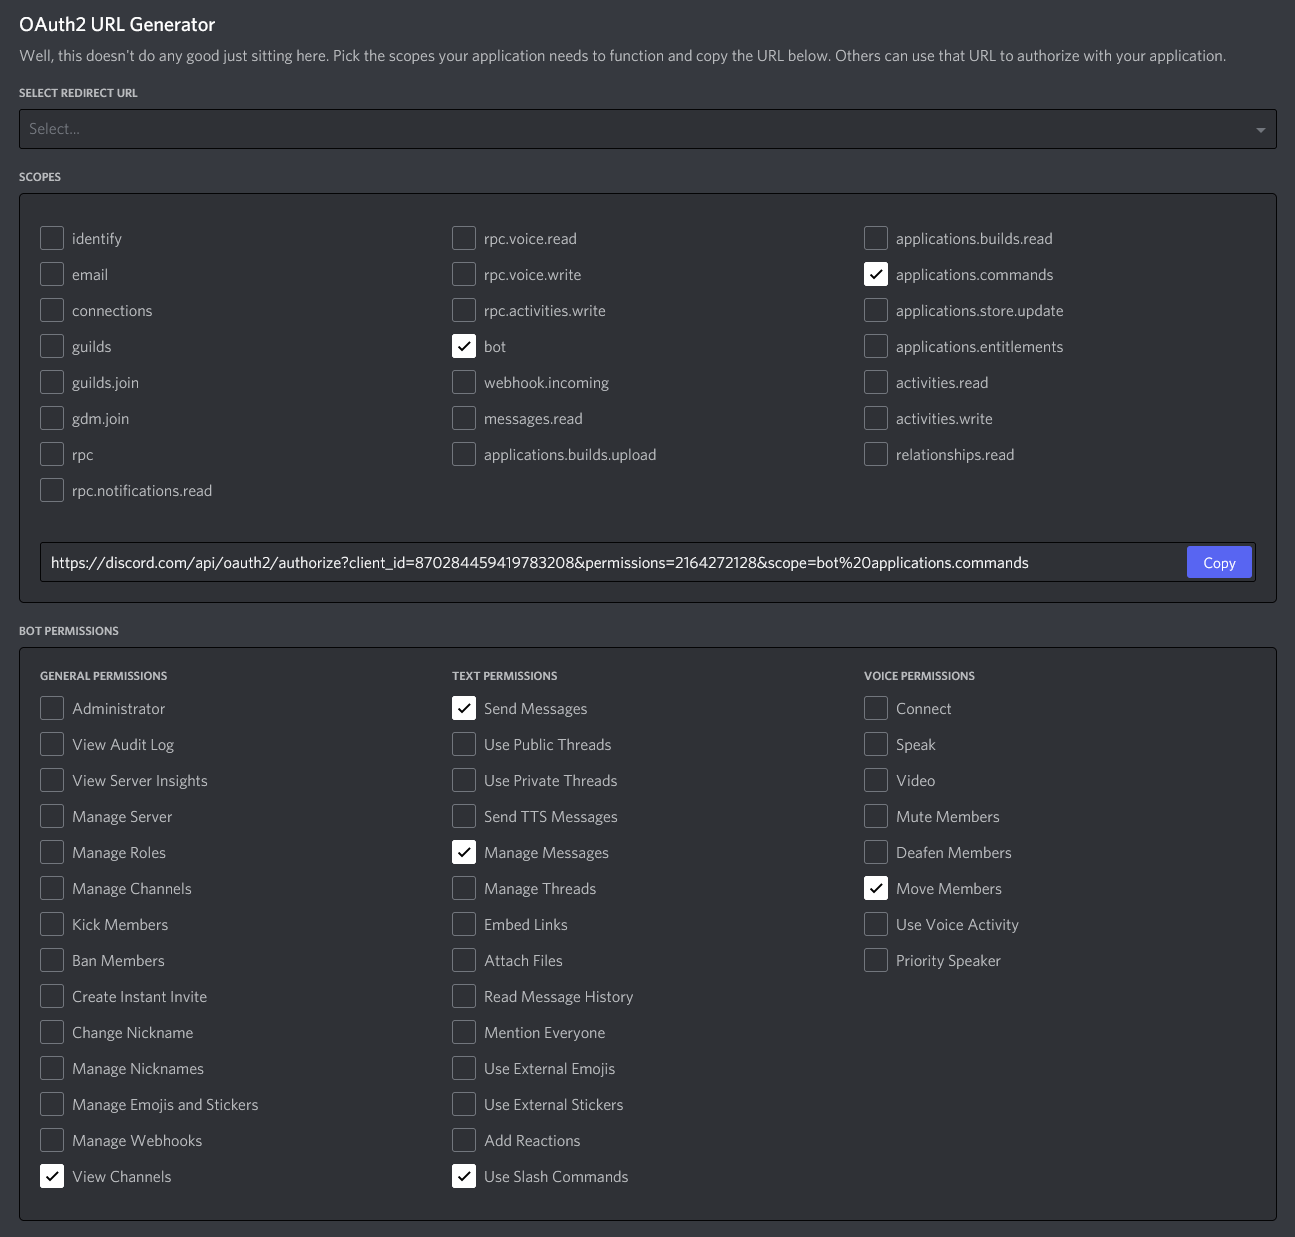
\includegraphics[width=15cm]{hosting_requirements/img3}
	}
	\item{
		Copy the generated URL and paste it into the .env file (see section \ref{hosting_requirements___prerequisites___the_.env_file}) as the value for key $INVITE\_URL$.
	}
	\item{
		Head over to the menu titled $Bot$ as seen below:\\\\
		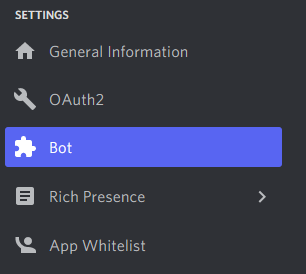
\includegraphics[width=8cm]{hosting_requirements/img4}
	}
	\item{
		Click the button labelled $Add Bot$, then click $Yes, do it!$.
	}
	\item{
		Click the button labelled $Copy$ which is located under $Click to Reveal Token$.
		Paste the contents into the $.env$ file (see section \ref{hosting_requirements___prerequisites___the_.env_file}) as the value for the key $DISCORD\_TOKEN$.
	}
	\item{
		Finally, navigate to the section titled $Privileged Gateway Intents$ and check both intents as seen below:\\\\
		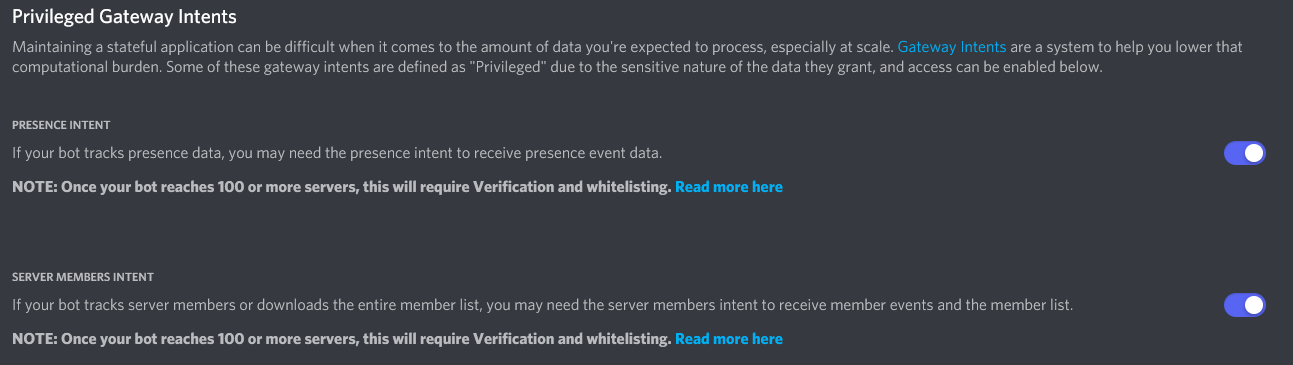
\includegraphics[width=15cm]{hosting_requirements/img5}
	}

\end{enumerate}

\subsubsection{The .env File}\label{hosting_requirements___prerequisites___the_.env_file}
This is a critical file that doesn't come with the git repo.
Its purpose is to contain environment variables such as the Discord Token which are sensitive therefore MUST NOT BE SHARED.
A template can be seen below:
\begin{verbatim}
DISCORD_TOKEN="<<your-token-here>>"
INVITE_URL="<<your-invite-url-here>>"
\end{verbatim}

\subsubsection{The newrelic.ini File}\label{hosting_requirements___prerequisites___the_newrelic.ini_file}
Demo Helper utilises New Relic to monitor the status of Demo Helper.
This isn't a requirement however and if you wanted to, you could remove the New Relic code and it won't impede Demo Helper performance.
However, if you want New Relic monitoring, then you will need a configuration file in the same place as the .env file.
A template can be seen below:
\begin{verbatim}
[newrelic]
license_key = <<your-license-key-here>>
app_name = Demo Helper
distributed_tracing.enabled = true
monitor_mode = true
log_level = info
ssl = true
high_security = false
transaction_tracer.enabled = true
transaction_tracer.transaction_threshold = apdex_f
transaction_tracer.record_sql = obfuscated
transaction_tracer.stack_trace_threshold = 0.5
transaction_tracer.explain_enabled = true
transaction_tracer.explain_threshold = 0.5
error_collector.enabled = true
browser_monitoring.auto_instrument = true
thread_profiler.enabled = true

# ---------------------------------------------------------------------------

[newrelic:development]
monitor_mode = false

[newrelic:test]
monitor_mode = false

[newrelic:staging]
app_name = Demo Helper (Staging)
monitor_mode = true

[newrelic:production]
monitor_mode = true

# ---------------------------------------------------------------------------
\end{verbatim}


\pagebreak
\subsection{Getting Demo Helper Onto Your Server}
The easiest way to go about doing this is to pull the git repository.
If you have git already installed then go ahead and run the following commands:
\begin{enumerate}
	\item{\texttt{sudo apt update}}
	\item{\texttt{sudo apt install -y git python3 python3-pip python3-dotenv}}
	\item{\texttt{git clone https://github.com/Amheus/DemoHelper}}
	\item{\texttt{pipenv install}}
\end{enumerate}

This will download almost everything you require to get Demo Helper running.
You will need to manually add two files as detailed in section \ref{hosting_requirements___prerequisites___the_.env_file} and section \ref{hosting_requirements___prerequisites___the_newrelic.ini_file}.


\pagebreak
\subsection{Running Demo Helper As A Service}
There are many ways you can go about doing this.
\subsubsection{Linux - Systemd}
\begin{enumerate}
	\item
	{
		Create the following file $/etc/systemd/system/DemoHelper.service$
		\begin{verbatim}
[Unit]
Description=Demo Helper
After=network.target
StartLimitIntervalSec=0

[Service]
Type=simple
Restart=always
RestartSec=1
User=<username>
WorkingDirectory=/home/<username>/DemoHelper
ExecStart=/usr/bin/pipenv run python3 -m DemoHelper

[Install]
WantedBy=multi-user.target
		\end{verbatim}
	}
	\item
	{
		Then run the following command to load in the configuration file we've just created.
		\begin{verbatim}
sudo systemctl daemon-reload
		\end{verbatim}
	}
	\item
	{
		Then to start the service, run the following command:
		\begin{verbatim}
sudo systemctl start DemoHelper
		\end{verbatim}
	}
\end{enumerate}
If you want Demo Helper to run on system startup, then run the following command:
\begin{verbatim}
sudo systemctl enable DemoHelper
\end{verbatim}

The following commands are used to manage a Systemd process.
\begin{itemize}
	\item
	{
		General
		\begin{itemize}
			\item
			{
				\texttt{sudo systemctl start DemoHelper}
			}
			\item
			{
				\texttt{sudo systemctl restart DemoHelper}
			}
			\item
			{
				\texttt{sudo systemctl stop DemoHelper}
			}
		\end{itemize}
	}
	\item
	{
		Monitoring 
		\begin{itemize}
			\item
			{
				\texttt{sudo systemctl status DemoHelper}
			}
			\item
			{
				\texttt{sudo journalctl -ru demohelper.service}
				\\Returns logs for the service.
			}
		\end{itemize}
	}
	\item
	{
		System Startup 
		\begin{itemize}
			\item
			{
				\texttt{sudo systemctl enable DemoHelper}
				\\Sets the service to automatically start on system startup.
			}
			\item
			{
				\texttt{sudo systemctl disable DemoHelper}
				\\Stops the service from automatically starting on system startup.
			}
		\end{itemize}
	}
\end{itemize}

\subsubsection{Linux - PM2}
To install Process Manager 2, run the following commands:
\begin{enumerate}
	\item{\texttt{sudo apt update}}
	\item{\texttt{sudo apt install -y npm}}
	\item{\texttt{sudo npm install pm2@latest -g}}
	\item{\texttt{cd ~/DemoHelper}}
	\item{\texttt{pm2 start main.py --name DemoHelper --interpreter python3}}
	\item{\texttt{pm2 save}}
	\item{\texttt{pm2 startup}}
\end{enumerate}

After a server reboot, run \texttt{pm2 resurrect} to bring back all process instances that were present when you ran \texttt{pm2 save}.

The following commands are used to manage a PM2 process:
\begin{itemize}
	\item
	{
		General
		\begin{itemize}
			\item
			{
				\texttt{pm2 start <pm2-id>}
			}
			\item
			{
				\texttt{pm2 restart <pm2-id>}
			}
			\item
			{
				\texttt{pm2 stop <pm2-id>}
			}
		\end{itemize}
	}
	\item
	{
		Monitoring 
		\begin{itemize}
			\item
			{
				\texttt{pm2 list}
				\\Returns a list of all processes managed by PM2.
			}
			\item
			{
				\texttt{pm2 monit}
				\\Similar to \texttt{pm2 list} but gives a more detailed overview
			}
			\item
			{
				\texttt{pm2 status <pm2-id>}
			}
		\end{itemize}
	}
	\item
	{
		System Startup 
		\begin{itemize}
			\item
			{
				\texttt{pm2 save}
			}
			\item
			{
				\texttt{pm2 startup}
			}
			\item
			{
				\texttt{pm2 resurrect}
			}
		\end{itemize}
	}
\end{itemize}



\pagebreak
\subsection{General Maintenance}
\begin{enumerate}
	\item{Update dependencies using \texttt{pipenv update}.}
	\item{Pull updates from the repository using \texttt{git pull}.}
	\item{Then restart the service.}
\end{enumerate}
	
